%% Bemærk:
%%          Resten af rapporten følger en stil hvor indledninger skrives
%%          med \sffamlily-typen. Denne stil bør også følges her.
%%

{\sffamily I dette afsnit vil vi afprøve den generelle metode for udtrækning af
regioner. Selve metodens fremgangsmåde står beskrevet i afsnit
\ref{section_udtraek}. Tærskelværdiern er sat til de fundne
tærskelværdier i afsnit \ref{terskelverdi}. Første del af afsnittet vil
omhandle afprøvning af metoden på testbilleder, og anden del afprøvning
ad metoden på udvalgte billeder fra databasen.}

\subsection{Afprøvning på test billeder}
I dette underafsnit afprøves metoden på billeder konstrueret med en hvis
baggrund og sorte regioner. Det snit, vi anvender,samt margin, er
indtegnet på testbillederne

I billedet \ref{GRD_test1} er der fem regioner. tre af dem bliver
fundet, da de ligger i snittet. De to regioner som ikke er fundet, er
stadig sorte. Som man kan se, bliver både den, der krydser snittet og den,
der tangere snittet, taget med. 

\begin{figure}[!h]
    \centering
    	\subfloat[Det originale malert.]{
	       	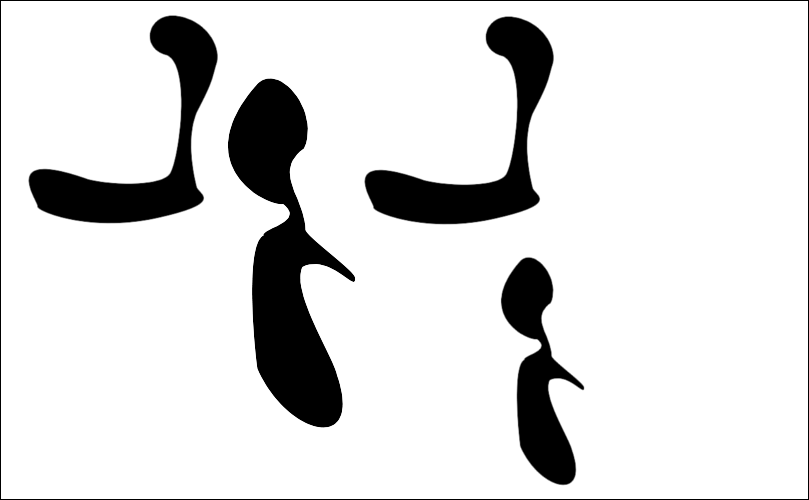
\includegraphics[angle=0,width=0.7\textwidth]{afsnit/afprovning/billeder/region_selector/blob_section.png}
	       	\label{GRD_test1_original}}\hspace{1em}
		\subfloat[Her ses fire regioner samt en baggrund. to af figurerne og baggrunden er blevet fundet af metoden.]{
        	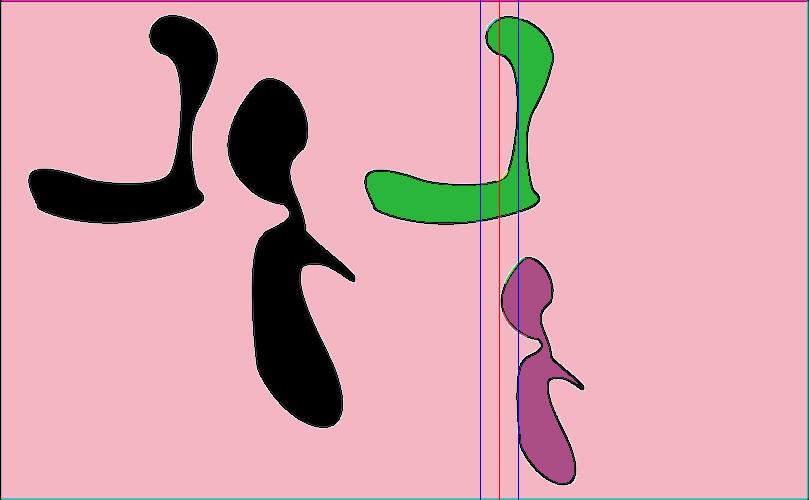
\includegraphics[angle=0,width=0.7\textwidth]{afsnit/afprovning/billeder/region_selector/blob_region_section.png}
        	\label{GRD_test1}}\hspace{1em}
        \caption[]{}
     \label{GRD_test1_sammen}
\end{figure}

I billedet \ref{GRD_test2} er der tre regioner, som
alle bliver fundet; Baggrunden, den lille region, som ligger inde for
margin, og den store region, som kun har en lille del af sin masse
i snittet. 

\begin{figure}[!h]
    \centering
    	\subfloat[Det originale malert.]{
	       	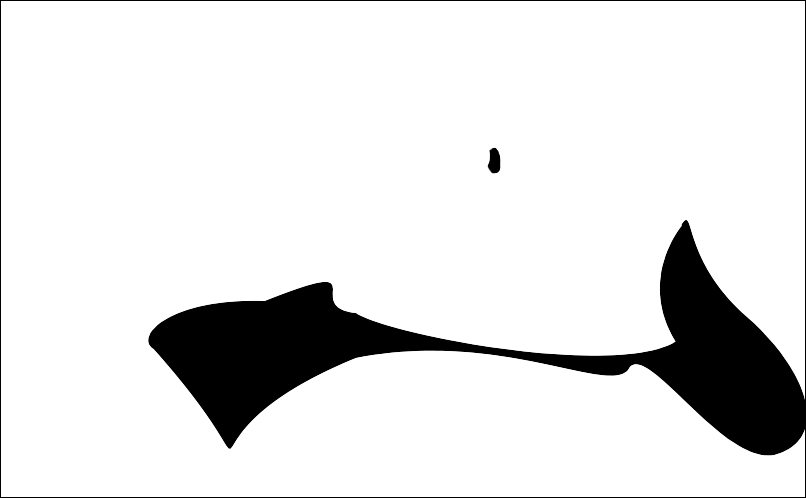
\includegraphics[angle=0,width=0.7\textwidth]{afsnit/afprovning/billeder/region_selector/lille_tvers.png}
	       	\label{GRD_test2_original}}\hspace{1em}
		\subfloat[På billedet er der fundet en stor og en mindre region]{
        	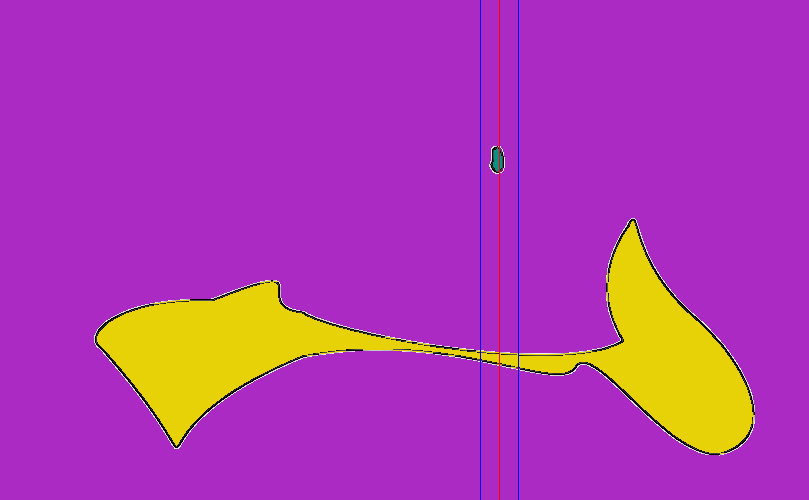
\includegraphics[angle=0,width=0.7\textwidth]{afsnit/afprovning/billeder/region_selector/blob2_region_section.png}
        	\label{GRD_test2}}\hspace{1em}
        \caption[]{}
     \label{GRD_test2_sammen}
\end{figure}

I billedet \ref{GRD_test3} er der en hoisont, som ligger oven på
snittet. Begge sider af hoisontlinien bliver udtrækket som en region.

\begin{figure}[!h]
    \centering
    	\subfloat[Det originale malert.]{
	       	
\includegraphics[angle=0,width=0.7\textwidth]{afsnit/afprovning/billeder/region_selector/hoisont.png}
	       	\label{GRD_test3_original}}\hspace{1em}
		\subfloat[På billedet er der fundet to store regioner]{
        	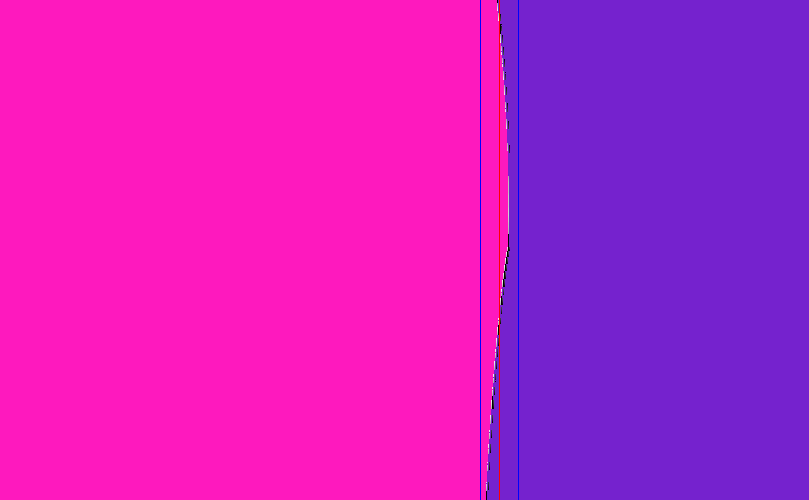
\includegraphics[angle=0,width=0.7\textwidth]{afsnit/afprovning/billeder/region_selector/hoisont_region_section.png}
        	\label{GRD_test3}}\hspace{1em}
        \caption[]{}
     \label{GRD_test3_sammen}
\end{figure}

I de tre figur \ref{GRD_test1_sammen}, \ref{GRD_test1_sammen} og
\ref{GRD_test1_sammen}, afbildes de tre billeder hvorpå metoden afprøves.
Metoden opføre sig efter de standarder, som vi fremsætte i afsnit \ref{section_naiv}, og
virker efter vores forventninger.
\clearpage

\subsection{Afprøvning på malerier}
Vi vil afprøve metoden til udtrækning af regioner på seks udvalgte
malerier. Malerierne skal demonstrere, hvordan metoden på nogle malerier
fungerer godt, mens den fungerer dårligt på andre

\begin{figure}[!h]
    \centering
		\subfloat[Maleri med Kraftige farver og få detaljer. Navn: Scenes from the Story of Joseph: The Arrest of His Brethren. År: 1515-16. Af: Bacchiacca.]{
        	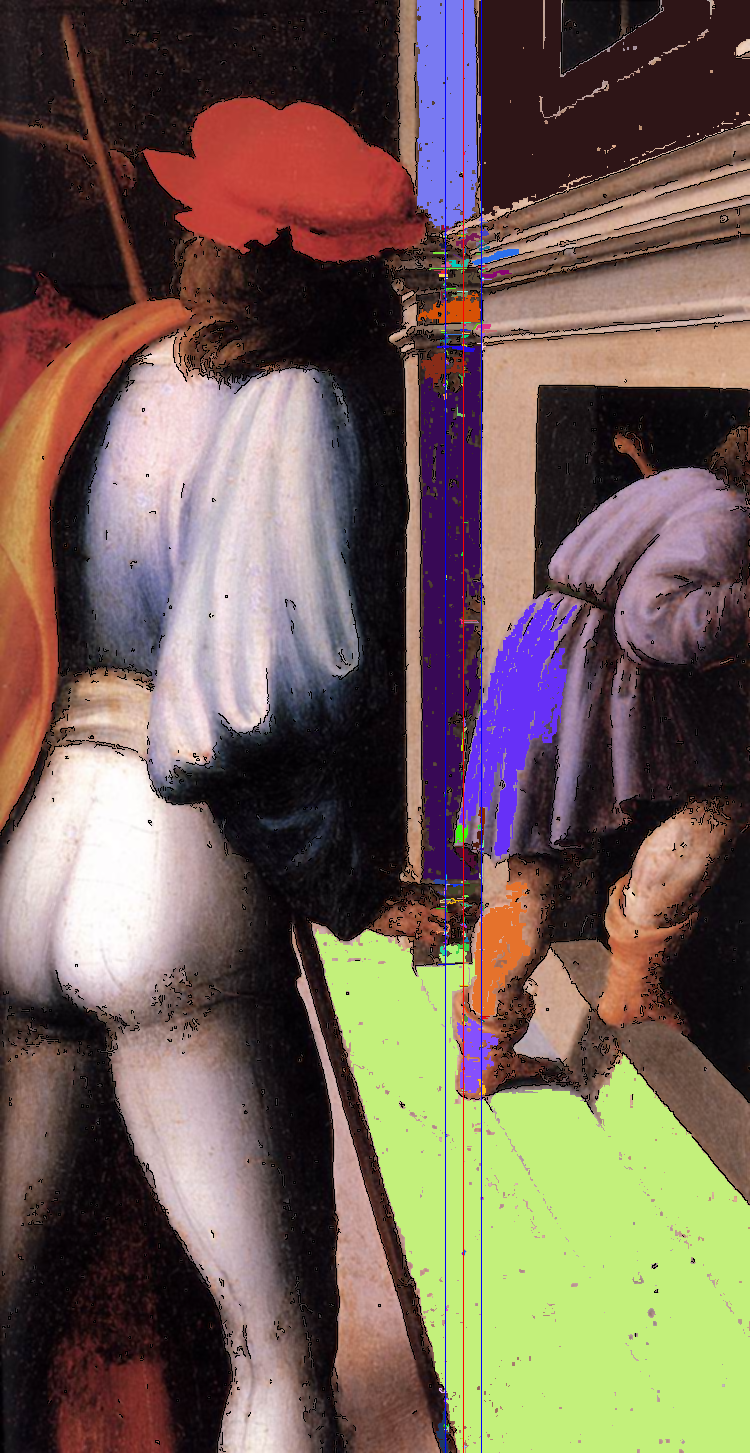
\includegraphics[angle=270,width=1.0\textwidth]{afsnit/afprovning/billeder/thressholds/krafitige_farver/svage_detalier/floodfill/4-4.png}
        	\label{GRD_virker1}}\hspace{1em}
		\subfloat[Maleri med middel kraftige farver og medium antal detaljer.]{
        	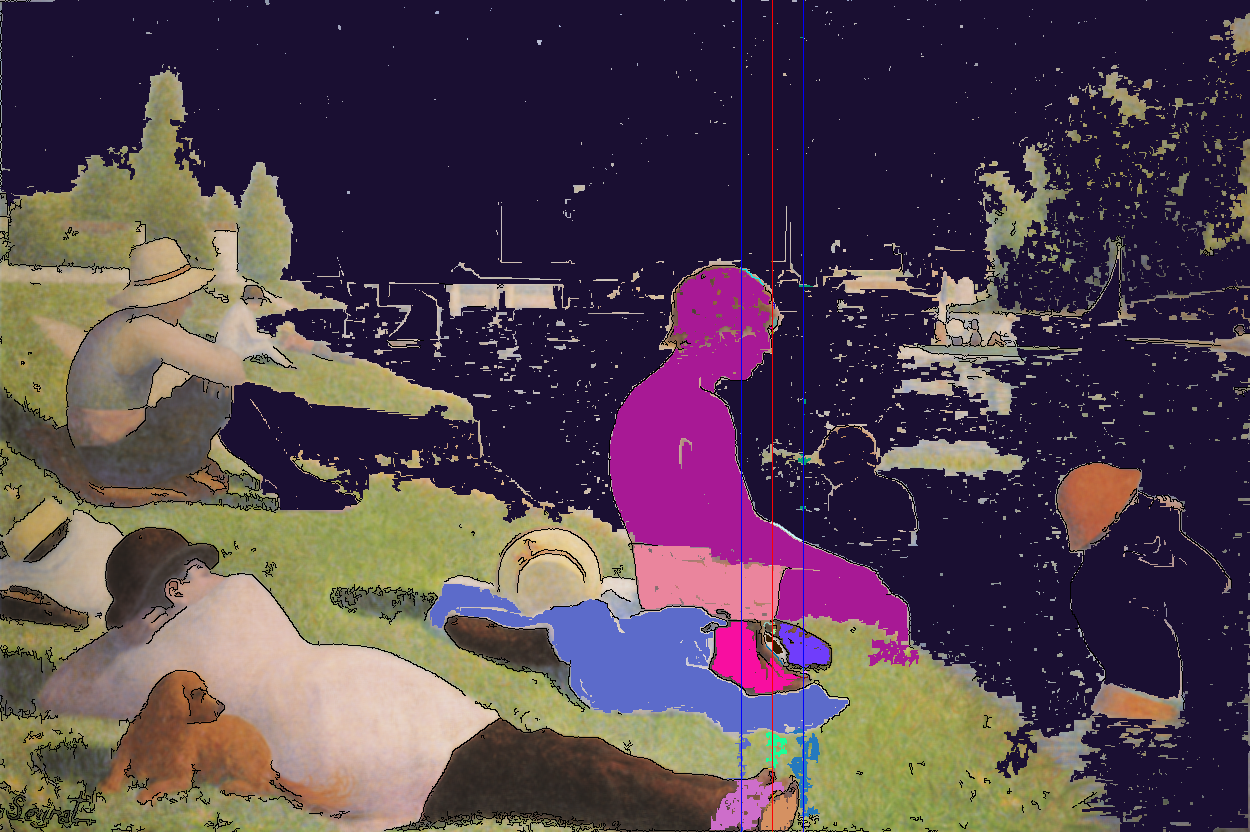
\includegraphics[angle=0,width=1.0\textwidth]{afsnit/afprovning/billeder/4-4.png}
        	\label{GRD_virker2}}\hspace{1em}
        \caption[]{2 malerier, hvor den generelle metode virker efter vores ønsker.}
     \label{generelde_region_detektor_virker}
\end{figure}

I figuren \ref{generelde_region_detektor_virker} er der to malerier, hvor
vores region detektor virker rigtige godt. 

I det første maleri \ref{GRD_virker1} finder metoden syv store regioner
samt en dele små. Den skelner mellem de forskellige paneler om kaminen,
og hvert stykke tøj på personen i maleriet opfattes som en særskilt
region. De små regioner er samlet, og forstyrre ikke de store regioner.
man kunne måske have ønsket sig, at metoden ville fylde mere af
personens kappe ud, men bortset fra det er figuren et godt eksempel på,
hvordan det ser ud, når den generelle metode fungerer.

I maleriet \ref{GRD_virker2} finder vi mange af de samme positive ting:
Drengen i midten af maleriet er helt udfyldt, en sko, drengens bade
bukser og et håndklæde er også fundet. Det er dog vigtigt at lægge mærke
til, at de andre personer i vandet, flyder i et med baggrunden. Dette
ville normalt være uheldigt, men eftersom metoden kun ser efter regioner
i snittet -repræsenteret ad den røde linje- gør det ikke noget i dette
tilfælde.

\begin{figure}[!h]
    \centering
	\subfloat[Maleri med kraftige farver og mange detaljer, hvor de tærskelværdierne fundet i afsnit \ref{terskelverdi} er brugt.]{
   	 	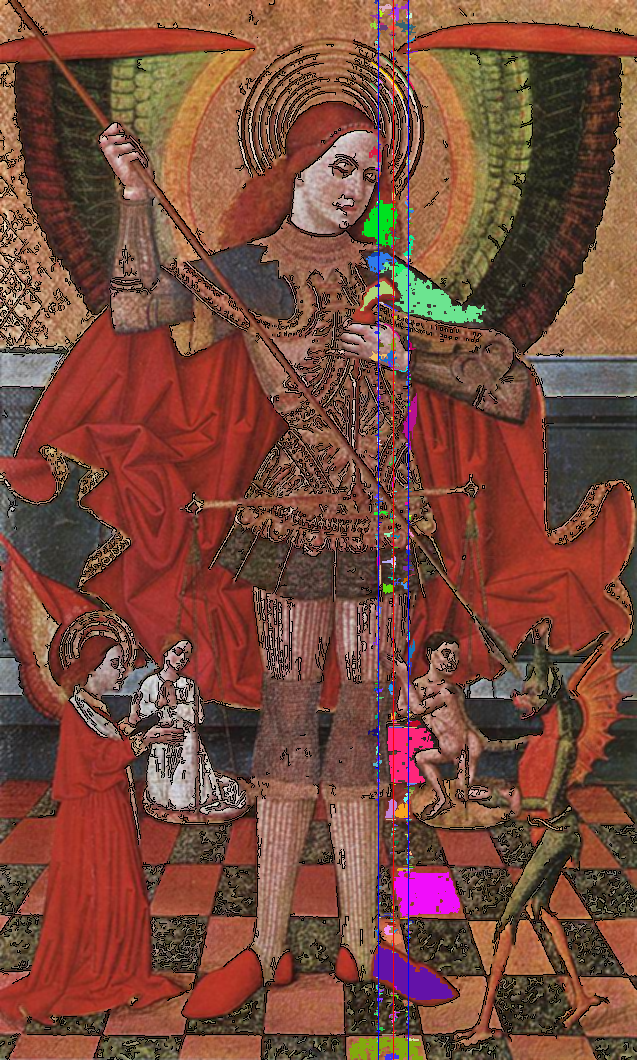
\includegraphics[angle=270,width=0.90\textwidth]{afsnit/afprovning/billeder/thressholds/krafitige_farver/krafite_detalier/floodfill/4-4.png}
	    \label{GRD_virker_nesten1}}\hspace{1em}
    \subfloat[Det samme maleri, hvor Tærskelværdier er valt specifikt for det her maleri]{
        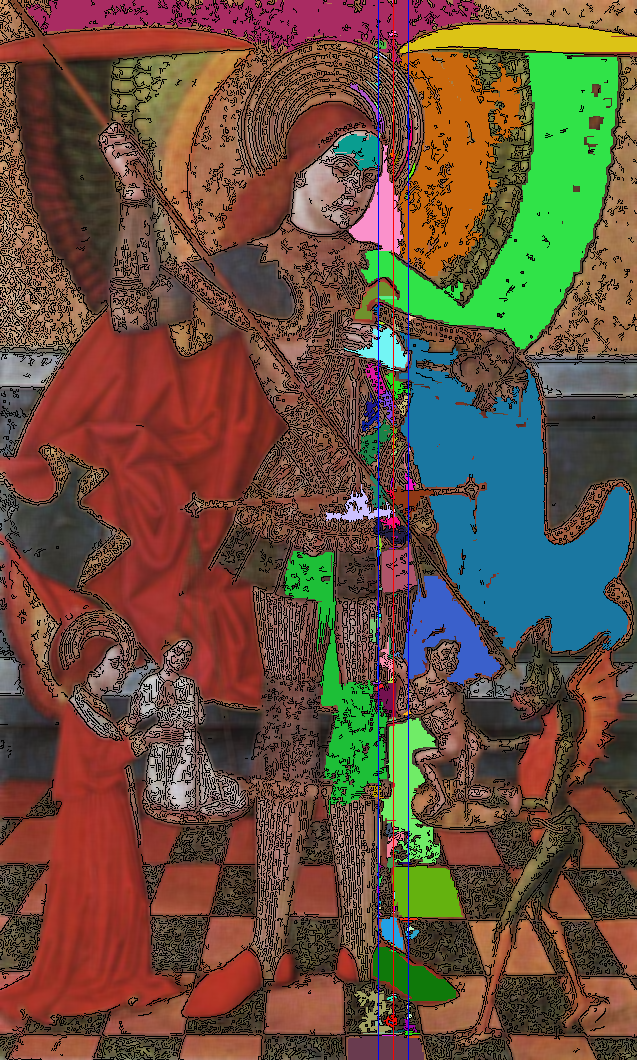
\includegraphics[angle=270,width=0.95\textwidth]{afsnit/afprovning/billeder/thressholds/krafitige_farver/krafite_detalier/s7_e200_f5.png}
        \label{GRD_virker_nesten1_super}}\\
     \caption[]{Et malerier, hvor den generelle metode ikke helt virker efter vores ønske, men med nye tærskelværider vil virker meget bedre}
     \label{generelde_region_detektor_virker_nesten1}
\end{figure}

\begin{figure}[!h]
    \centering
    \subfloat[Maleri med middel kraftige farver og medium antal detaljer.]{
        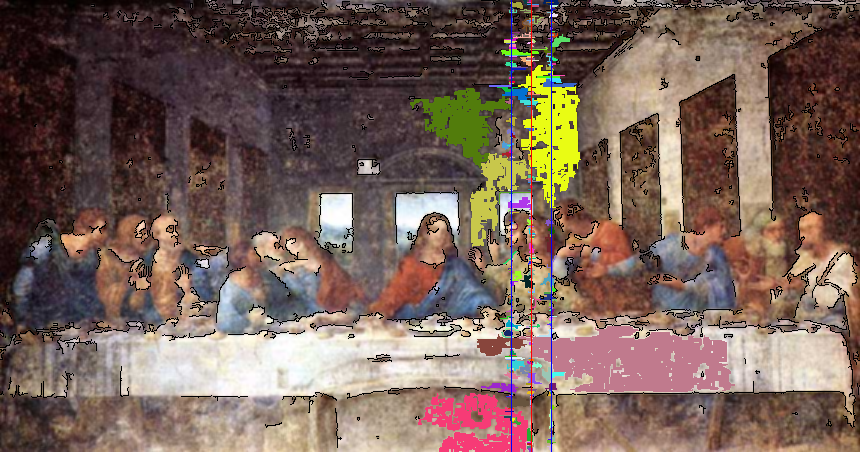
\includegraphics[angle=0,width=0.95\textwidth]{afsnit/afprovning/billeder/thressholds/medium_farver/medium_detalier/floodfill/4-4.png}
        \label{GRD_virker_nesten2}}\\
	\subfloat[Det samme maleri, hvor Tærskelværdier er valt specifikt for det her maleri]{
   	 	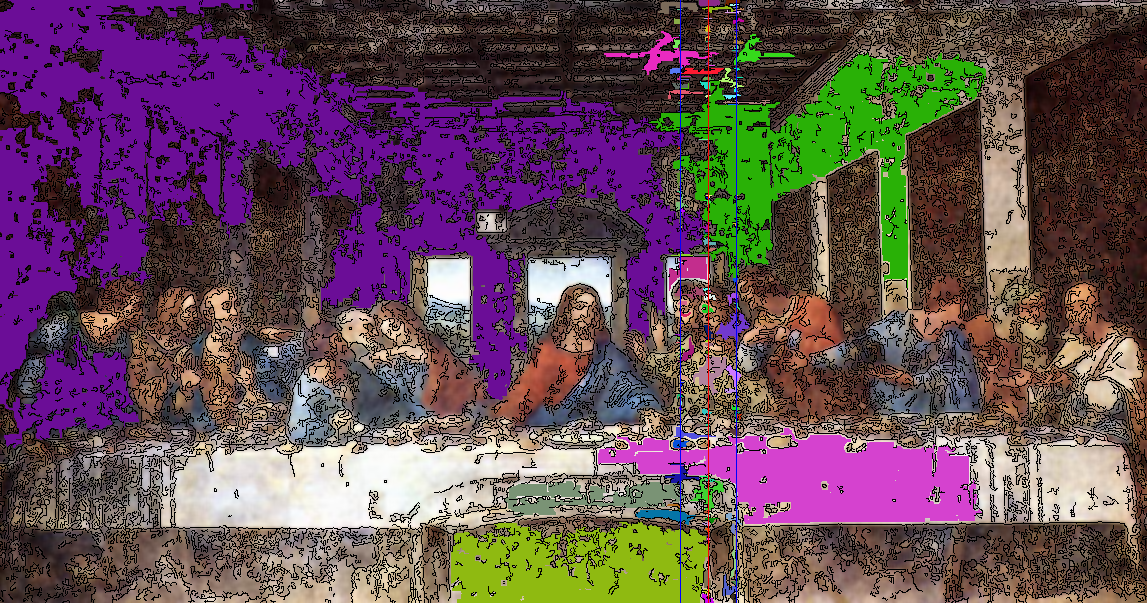
\includegraphics[angle=0,width=0.90\textwidth]{afsnit/afprovning/billeder/thressholds/medium_farver/medium_detalier/s5_e90_e200_f4.png}
	    \label{GRD_virker_nesten2_super}}\hspace{1em}
     \caption[]{Et malerier, hvor den generelle metode ikke helt virker efter vores ønske, men med nye tærskelværdier vil virker meget bedre}
     \label{generelde_region_detektor_virker_nesten2}
\end{figure}

I figur \ref{generelde_region_detektor_virker_nesten1} og \ref{generelde_region_detektor_virker_nesten2} er der to
malerier, hvor metoden ikke fungerer optimalt efter hensigten. Dog kan
vi stadig bruge figurerne til noget

I maleriet \ref{GRD_virker_nesten1} bliver der mest fundet flest små
regioner. En sko, en skulder og en flise trækkes ud, hvor vi hellere
ville have haft, at personens kappe og arm blev fundet. Dette skyldes
primært, at tærskelværdierne for dette billede er sat for lavt. 


Maleriet i den anden figur \ref{GRD_virker_nesten2} rummer nogle af de
samme problemer: Metoden finder også her en masse små dele af figurer,
der burde hænge sammen. Det vil også kunne løses ved nogle andre
tærskelværdier, men som man også kan se på maleriet er væge og loftet -
som egentlig er ret ensfarvede -stadig svære at finde for metoden. Det
kunne tyde på, at en højere grad af sløring ville løse problemet, og få
algoritmen til at virke i maleriet.

Når netop de to figure \ref{GRD_virker_nesten1} og
\ref{GRD_virker_nesten2} er interessante, er det fordi, at en ændring af
tærskelværdier, samt en højre grad af sløring, ville bevirke, at den
generelle metode kom til at fungere bedre. I billedet
\ref{GRD_virker_nesten1_super} og \ref{GRD_virker_nesten1_super} er
protretere de samme malerier, men hvor tærskelværdierne passer bedre til
maleriet, man kan se det ved f.eks at karben på anglen samt det meste af
loftet bliver fundet.

\clearpage

\begin{figure}[!h]
    \centering
     \subfloat[Det originale billedet. Navn:Vase of Flower. År: ukent. Af: Arellano, Juan de]{
        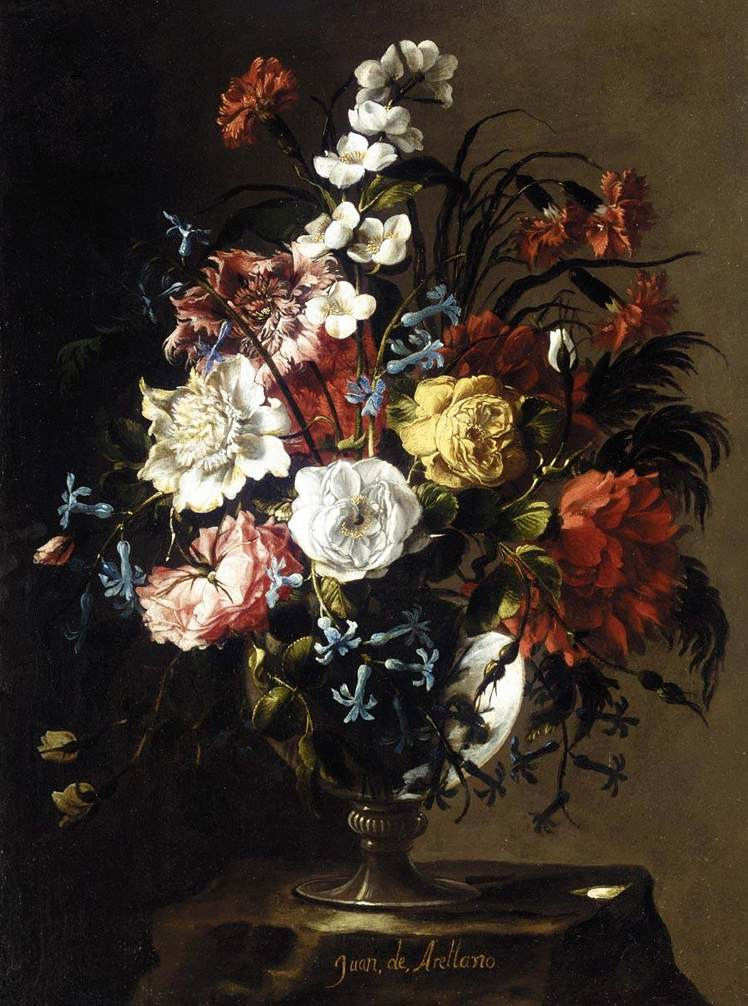
\includegraphics[angle=0,width=0.46\textwidth]{afsnit/afprovning/billeder/thressholds/krafitige_farver/medium_detalier/mDetalier}
        \label{GRD_virker_ikke1_orginal}}
    \subfloat[Maleri med Kraftige farver og medium detaljer.]{
        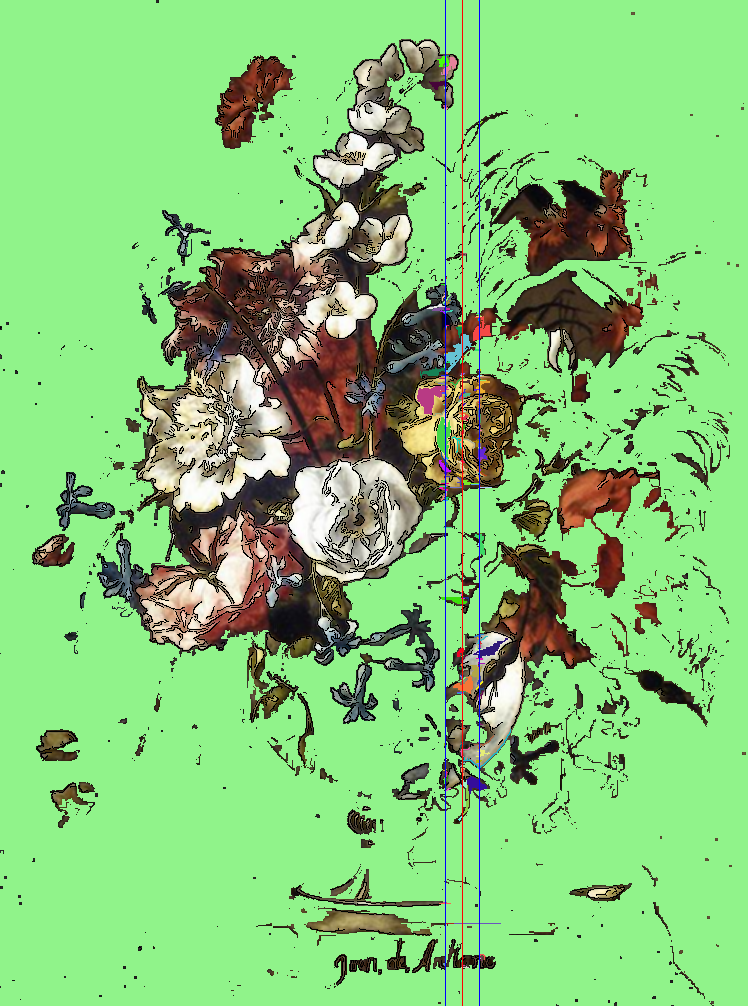
\includegraphics[angle=0,width=0.46\textwidth]{afsnit/afprovning/billeder/thressholds/krafitige_farver/medium_detalier/floodfill/4-4.png}
        \label{GRD_virker_ikke1}}
     \caption{Maleri af blomster, hvor den generelde metode ikke virker}
     \label{generelde_region_detektor_virker_ikke}
\end{figure}

\begin{figure}[!h]
	\begin{center}
	    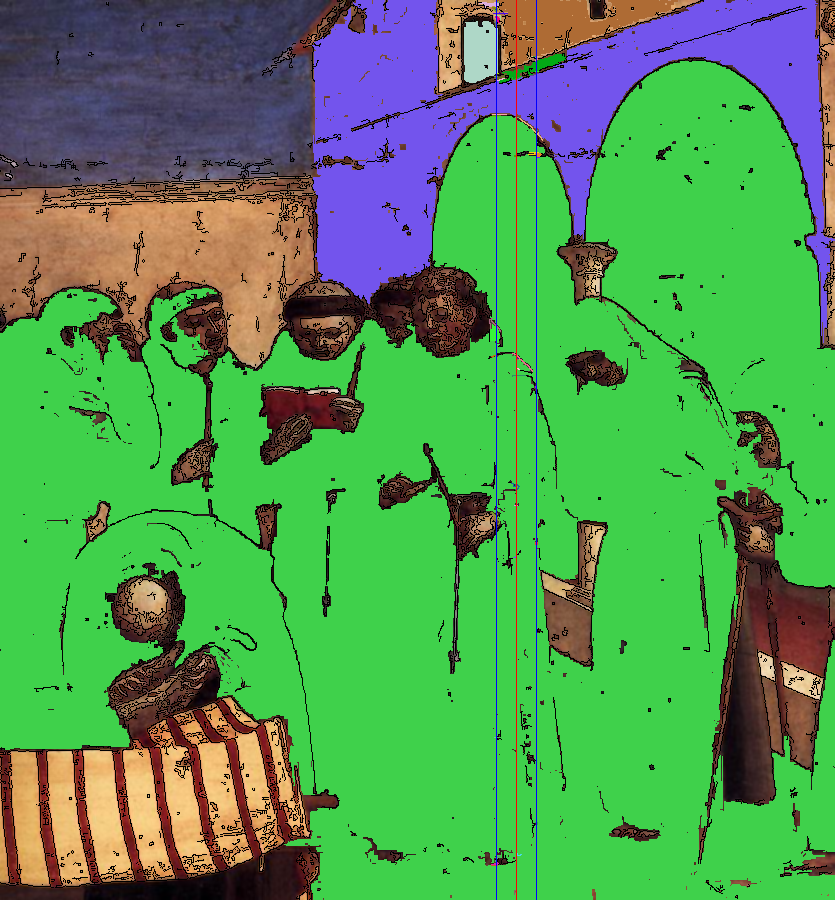
\includegraphics[angle=0,width=0.65\textwidth]{afsnit/afprovning/billeder/thressholds/svage_farver/svage_detalier/floodfill/4-4.png}
	\end{center}    
	\caption{Maleri med svage farver og få detaljer.}
    \label{GRD_virker_ikke2}
\end{figure}

I figur \ref{generelde_region_detektor_virker_ikke} og
\ref{GRD_virker_ikke2} er der to malerier hvor
vores generelle metode ikke virker optimalt. 

I maleri \ref{GRD_virker_ikke1} er noget af buketten og baggrunden gået
i et. Desuden er resten af blomsterne i snittet ikke fyldt ud, og selv
en ændring i tærskelværdierne vil ikke hjælpe, da en øgning af disse
blot vil resultere i, at flere af blomsterne går i ét med baggrunden. En
sænkning vil resultere i, at ingen af blomsterne bliver trukket ud. 

Maleriet \ref{GRD_virker_ikke2} repræsenterer en anden problemstilling,
som vi ikke kan komme udenom: Farverne er så mørke og svage, at en
ændring i tærskelværdien i floodfill på bare en vil få metoden til at gå
fra at finde ingen regioner til at finde for store regioner. det kan ses
i figur \ref{ff_munke}, hvor de 2 malerier, hvor floodfills tærskelværdi
er sat til den lavest og næst laves værdi. Som man kan se, finde metoden
mange snå regioner som ikke er særlige intrasant i maleri
\ref{munk_etff}, men i \ref{munk_toff}, bliver der fundet 2 meget store
regioner, som er blevet alt for store. Dette er et problem da vi så ikke
kan have en tærskelværdi som virker.

\begin{figure}[!h]
    \centering
     \subfloat[Tærskelværdierne for floordfill på maleriet er sat til en]{
        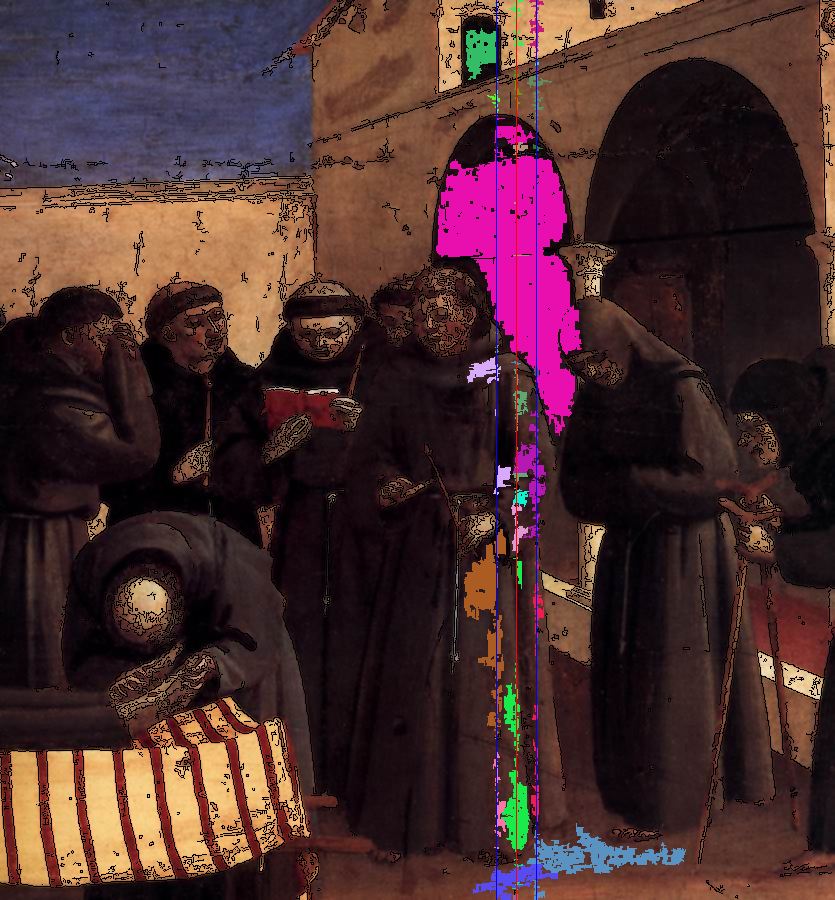
\includegraphics[angle=0,width=0.46\textwidth]{afsnit/afprovning/billeder/thressholds/svage_farver/svage_detalier/1-1.png}
        \label{munk_etff}}
    \subfloat[Tærskelværdierne for floodfill på maleriet er sat til to]{
        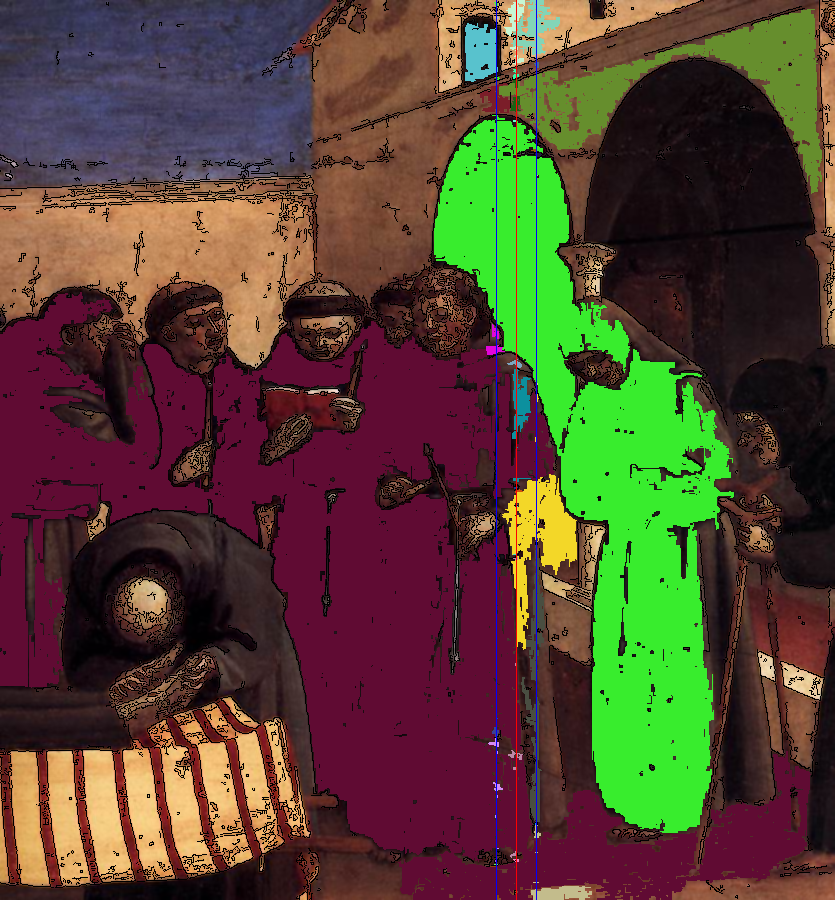
\includegraphics[angle=0,width=0.46\textwidth]{afsnit/afprovning/billeder/thressholds/svage_farver/svage_detalier/2-2.png}
        \label{munk_toff}}
     \caption{Et maleri hvor tærskelværdien for floodfill er sat til den laveste værdi den kan have, og et hvor denne næst laves tærskelværdien er sat.}
     \label{ff_munke}
\end{figure}

Dette kan også skyldes, at kantdetektionen tilføjer en mørk kant rundt
om regionerne, men da maleriet er mørkt i forvejen, hjælper
kandetektionen ikke. I maleri \ref{bla} er kanten tegnet med blåt og man
kan se at munken to fra venstre, ikke får sit skæg med, men hvor han går
det i maleriet med sort kant, se maleri \ref{sort}.

\begin{figure}[!h]
    \centering
     \subfloat[Maleri med blå kanter i kantdetektionen]{
        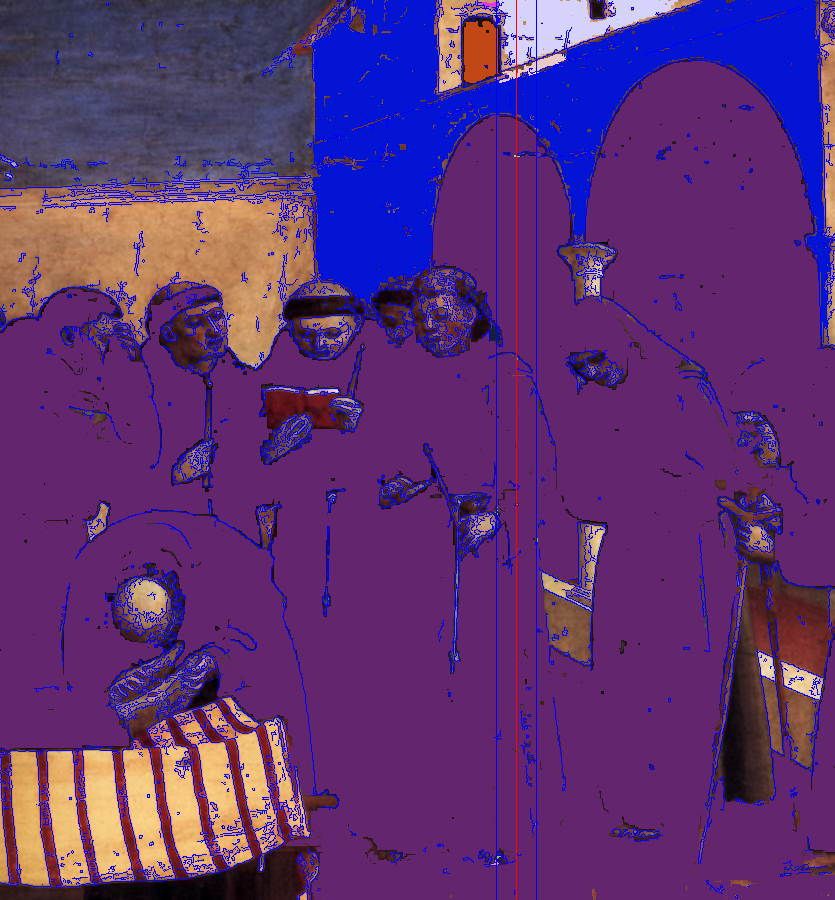
\includegraphics[angle=0,width=0.46\textwidth]{afsnit/afprovning/billeder/thressholds/svage_farver/svage_detalier/blueE.png}
        \label{bla}}
    \subfloat[Maleri med sorte kanter i kantdetektionen]{
        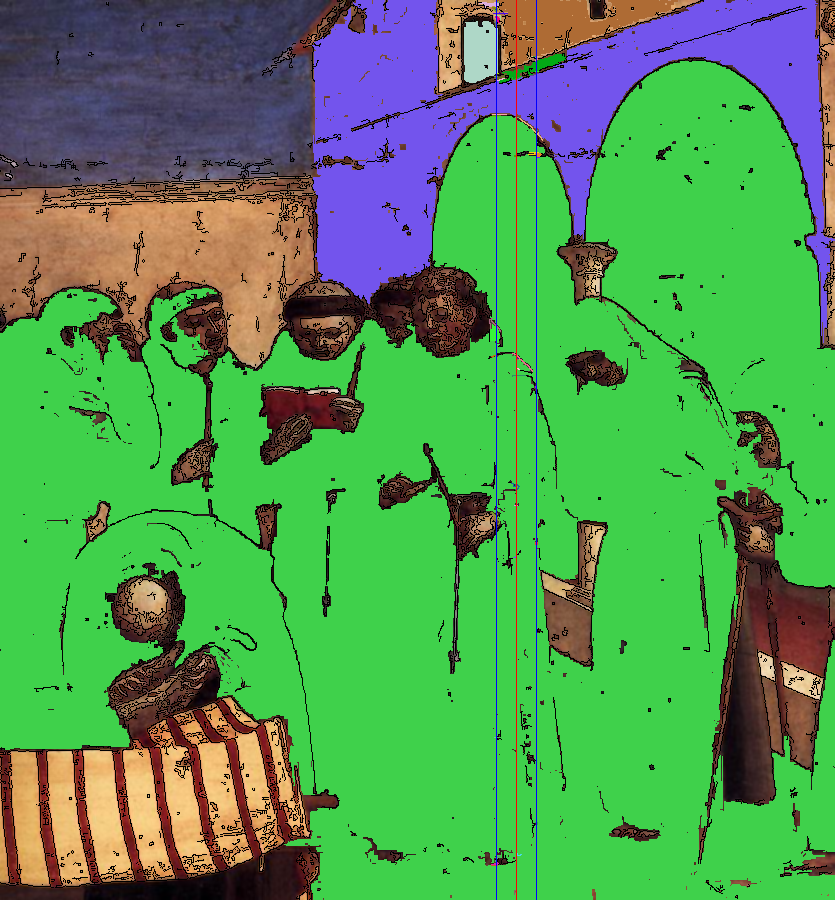
\includegraphics[angle=0,width=0.46\textwidth]{afsnit/afprovning/billeder/thressholds/svage_farver/svage_detalier/floodfill/4-4.png}
        \label{sort}}
     \caption{To forskellige farver brugt til at ligge kanter på maleriernes regioner}
     \label{fleremunke}
\end{figure}

